\documentclass[11pt,twocolumn]{asaproc}

\usepackage{graphicx}
\graphicspath{{images/}}

\usepackage{amsmath}
\usepackage{url}
\usepackage{numberedblock}

%\usepackage{mathtime}

%%UNCOMMENT following line if you have package
\usepackage{times}

\title{Bayesian Analysis of COVID-19 cases in California}

\author{Gulzina Kuttubekova\thanks{UCSC Baskin School of Engineering, Department of Statistical Science}}
\begin{document}


\maketitle





\begin{abstract}
 Since mid-January of 2020, we have seen the first cases of coronavirus disease (COVID-19) in the US. Serious respiratory disease caused by the novel virus had taken the lives of approximately 300,000 people in the world and infected more than 4.3 million people worldwide. \url{https://www.worldometers.info/coronavirus/} provides various COVID-19 related statistics about the US as well.

% write what you will do here
We examine the dataset of COVID-19 cases in California, along with the death rate among those who were found infected by this novel virus. We also look for a possible correlation between the number of infected people and the population in each county. We employ two hierarchical models to examine the infection rate and assess models by posterior predictive checks. 

% results
A modified hierarchical model on the joint distribution of the number of infections and the number of deaths showed a better fit than the hierarchical model which doesn't take into account the mortality rate and its distribution. In general, we saw systematic differences in the number of deaths and infections across counties. The assumption that the mean number of the number of infections is 20\% of the population had a high impact on the posterior distribution in the first model.


\begin{keywords}
Bayesian analysis, COVID-19, hierarchical models, MCMC
\end{keywords}
\end{abstract}







\section{Introduction\label{Introduction}}

% Intro - motivation
 The novel virus is still spreading across the world despite the precautions taken by governments of different countries. The numbers connected to this pandemic are changing very rapidly, not every day, but every hour.  There are only 13 countries left where there are no officially confirmed cases of COVID-19, according to \url{https://www.aljazeera.com/news/}. However, it's believed that it's only a matter of time while the novel virus reaches those countries. Since the first massive cases of COVID-19 and related death numbers started increasing in the Greater Seattle area in the US in mid-March, the epicenter of outbreak shifted quickly from West to East coast. At the current time, the Greater New York area became the epicenter of coronavirus battle. Although the state of California has as twice as the population as New York state, according to Worldometers number of reported infected people in the New York area is seven times greater than in California. Obviously there are many external factors that can explain this discrepancy.
 
%Problem
We want to know if there exists any discrepancy in the distribution of COVID-19 cases among the counties in California. If yes, which counties are more influential in explaining the number of death per reported number of infected people. We are also interested in the variation in the number of infected people by county. It's expected that as larger the population of the county as greater the number of infected people. However, it might be a false expectation, since there are other factors influencing the infection rate as population density, social culture, access to healthcare services and etc. We also integrate the new assumption that infection depends on mortality to answer the proposed research questions.

%What we employ/do?
We employ two hierarchical Poisson models constructed in different ways. We tackle the problem stated above using a fully Bayesian approach. Results from those models are reported and compared. We also use results from the previous study, which are available at \url{https://github.com/kgulzina/bayesian-analysis-of-COVID19-in-CA} for additional model checks.




\subsection{Data}

% Describe dataset
We analyze the dataset which contains information about incidence and mortality due to coronavirus in California. The number of reported cases and death is given per each county as of 04/13/2020. There are 58 observations, as there are 58 counties in the state in total. There are 4 variables: \{County, Total.cases, Deaths, Population\} s.t. population, the number of infected people, and number of people who died from COVID-19 are given. As we have count variables except for the county name, we treat the number of deaths $y_i$  out of $n_i$ infected people per $i^{th}$ county with population $c_i$ as discrete random variables. We also treat $y_i$ and $n_i$ as response variables.


\subsection{EDA}
The top three counties with the largest number of infected people are Los Angeles, San Diego, and Riverside.  Although San Francisco county has the largest population density $\sim18,553$, among all 58 counties in the state, it has 11 times less number of infected people compared to Los Angeles county with $\sim2,488$ population density. There are five counties that have zero reported cases of COVID-19. All five counties have population $\leq 32,000$. Interestingly four of those counties are in Northern California, and Mariposa county is relatively close to the highly populated county like Santa Clara. Up to date, $\sim 0.06\%$ of the population of California were infected with the virus. We would like to learn the trend in the number of deaths as this percentage increases. Moreover, throughout the study, we assume the mean number of coronavirus cases is equal to 20\% of the population. 

% include plot1: case numbers
\begin{figure}[t]
\centering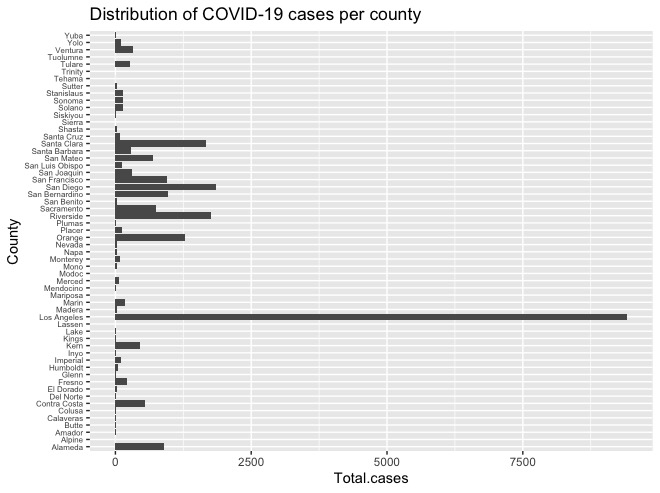
\includegraphics[scale=.30]{infected_per_county.jpeg}
\caption{Distribution of the total number of confirmed cases of COVID-19 across counties of California.}
\label{fig:totcases}
\end{figure}

% include plot2: case numbers by population
\begin{figure}[t]
\centering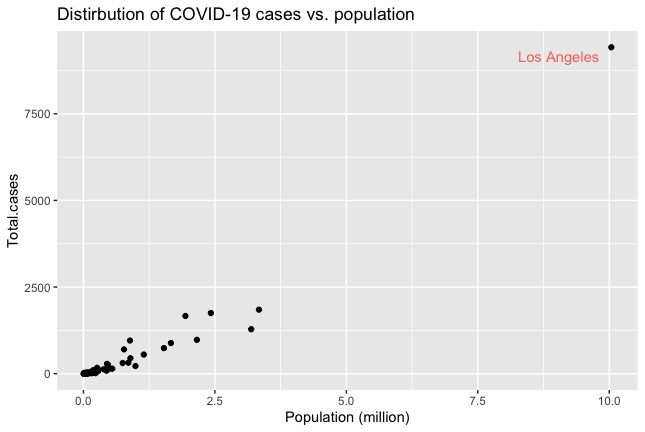
\includegraphics[scale=.31]{inf_vs_pop.jpeg}
\caption{Scatter plot number of confirmed cases of COVID-19 vs population for each county in California.}
\label{fig:infpop}
\end{figure}

% talk about infection rate vs population
According to the plot in Figure ~\ref{fig:totcases}, we see that number of confirmed cases is not evenly distributed across counties. Los Angeles has the most noticeable spike in cases. The top five counties with the total number of infected people $\geq$ 1,000 are Los Angeles, San Diego, Riverside, Santa Clara, and Orange counties. Apparently these high numbers are associated with the population in each county. Figure ~\ref{fig:infpop} shows that as population number increases the number of infected people increases as well. Scatter plot shows there is a potential outlier: Los Angeles county, which has the largest population and the highest number of infected people as well. As we stated earlier, there might be some other external factors affecting the non-homogenous distribution of cases across counties. For instance, infection numbers can be related to population density as we see in Figure ~\ref{fig:density},  the top 5 infected counties have population density of $\geq$ 1,000. Note that in the previous study we treated the number of confirmed cases $n_i$ as a known quantity, and now we treat it as a random variable of interest. 

% include plot3: population density of California counties
\begin{figure}[t]
\centering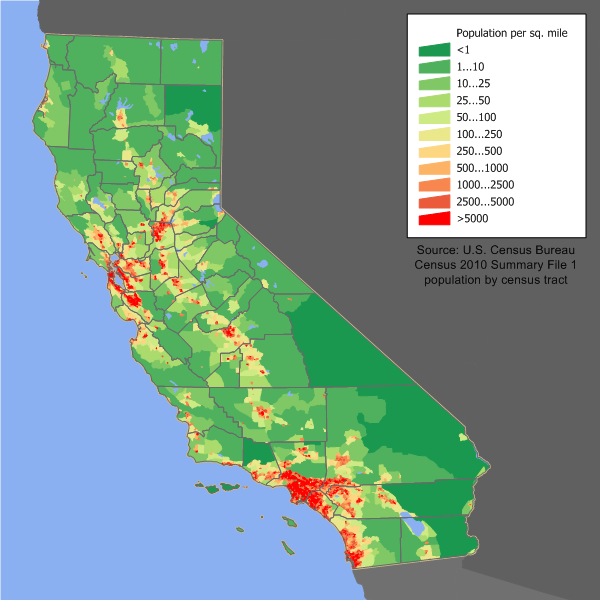
\includegraphics[scale=.30]{density.png}
\caption{Population density of California (Hines 2019).}
\label{fig:density}
\end{figure}

% include plot4: death rate per infected
\begin{figure}[t]
\centering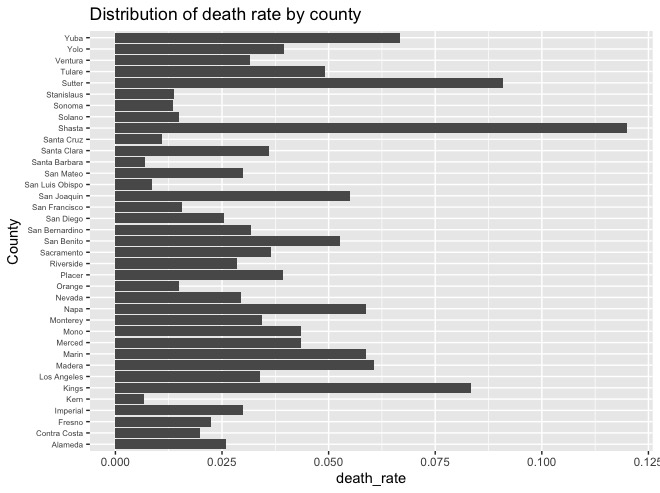
\includegraphics[scale=.30]{death_rate.jpeg}
\caption{Distribution of death rate due to COVID-19 across counties of California.}
\label{fig:deathrate}
\end{figure}

% talk about death rate per county explained by population:
Figure ~\ref{fig:deathrate} shows that the death rate, i.e. the proportion of deaths per confirmed coronavirus cases are far from being the same. For instance, Shasta, Sutter, and Kings counties have a greater mortality rate than in Los Angeles county. Even if we see this discrepancy, we can argue and treat the death rate to be the same across counties. The answer is obvious: since we don't have enough observations of confirmed cases in small populated counties like Sutter ($\leq 100,000$) empirical estimate of proportion may give misleading information about the true death rate. For instance, assume there is a county that has only 10 confirmed cases of COVID-19, by chance 2 people have serious underlying illnesses and those two patients die. Then the empirical estimate of proportion is 0.2! Which is greater than the sample death rate in any other county. 

Our preliminary findings suggest that the distribution of total cases of coronavirus differ by counties. Although we assume that the death rate is the same across counties, we test it by employing different models. In the next section, we describe models in detail.








\section{Methods}

% state the variables by detail
As stated before, number of death $y_i$ out of $n_i$ infected people per county $i$ are independent observations from Binomial distribution conditioning on $\theta_i = P(death)$. Also, population of each county $c_i$ is considered as an explanatory variable for modeling distribution of number of infections $n_i$. 



\subsection{Hierarchical Poisson model with Gamma priors}
First, we consider a model: 
$$n_i \sim Poi(\lambda_i c_i/10^3)$$
$$\lambda_i \sim Ga(\alpha, \beta)$$
$$p(\alpha, \beta) = Ga(\alpha |a_{\alpha}, b_{\alpha})Ga(\beta | a_{\beta}, b_{\beta})$$

where prior and hyperprior distributions have $Ga(shape, scale)$ structure and all parameters are greater than zero. 

We set the values of hyperparameters of the hyperprior distribution $p(\alpha, \beta)$ according to the assumption that, for a given county, the mean number of cases is equal to 20\% of the population. To include this assumption we do the following procedure:

\begin{enumerate}
\item For county $i$, $$E[n_i | \lambda_i] = \lambda_i c_i/10^3 = 0.2c_i$$ $$\lambda_i = 200$$
\item Assuming that distribution of $\lambda$ should be concentrated around 200, we set $$E[\lambda_i|\alpha, \beta] = \alpha\beta = 200$$
\item Then we let $$E[\alpha|a_{\alpha}, b_{\alpha}] = a_{\alpha}b_{\alpha} = 20 $$ $$E[\beta|a_{\beta}, b_{\beta}] = a_{\beta}b_{\beta} =10 $$
\item Consequently, we set $a_{\alpha} = 10, b_{\alpha} = 2, a_{\beta} = 20, b_{\beta} = 0.5$. 
\end{enumerate}

We write the posterior distribution as $$p(\mathbf{\lambda}, \alpha, \beta| \mathbf{n}) = p(\mathbf{\lambda}|\alpha, \beta, \mathbf{n})p(\alpha, \beta| \mathbf{n})$$ 

We can also write $p(\mathbf{\lambda, \alpha, \beta}| \mathbf{n})$: 
\begin{align*}
& \propto p(\alpha, \beta)p(\mathbf{\lambda}|\alpha, \beta)p(\mathbf{n}|\mathbf{\lambda}) \\
&\propto p(\alpha, \beta)\prod_{i=1}^{58}Ga({\lambda_i|\alpha, \beta})Poi(n_i|\frac{\lambda_i c_i}{10^3})
\end{align*}

Using this joint posterior we get the full conditional distribution of $\lambda: p(\lambda|-)$
$$p(\mathbf{\lambda}|\alpha, \beta, \mathbf{n}) = \prod_{i=1}^{58}p(\lambda_i|\alpha, \beta, n_i)$$ 
$$p(\lambda_i|\alpha, \beta, n_i) = Ga(\alpha + n_i, \big{(}\frac{1}{\beta} + \frac{c_i}{10^3}\big{)}^{-1})$$

Now we have to find $p(\alpha, \beta| \mathbf{n})$: 
$$p(\alpha, \beta| \mathbf{n}) \propto p(\alpha, \beta)p(\mathbf{n}|\alpha, \beta)$$

where $p(\mathbf{n}|\alpha, \beta) = \prod_{i=1}^{58}p(n_i|\alpha, \beta)$ and 

\begin{align*}
p(n_i|\alpha, \beta) & = \int p(n_i|\lambda_i)p(\lambda_i|\alpha, \beta) d\lambda_i \\
& = \int Poi(n_i|\frac{\lambda_ic_i }{10^3})Ga(\lambda_i | \alpha, \beta) d\lambda_i \\
& = \frac{\tilde{c}_i^{n_i}\Gamma(\alpha+n_i)}{n_i!\Gamma(\alpha)\beta^{\alpha}} (\frac{1}{\frac{1}{\beta} + \tilde{c}_i})^{(\alpha+n_i)}
\end{align*}

where $\tilde{c_i} = c_i/10^3$.

% Write the sampling procedure here:
We use this factorization to sample from the joint posterior distribution. First, we use \texttt{sample()} function in R and Griddy sampling approach to sample from $p(\alpha, \beta | \mathbf{n})$ and using those samples, we directly draw $\lambda_i$ from $Ga(\lambda_i|-)$ for each $i = 1, ..., 58$. Further, we get point and interval estimates of posterior mean and posterior variance using that sample for each parameter.

% How will you assess the model? Write model checking compared with results from previous study
We also obtain samples from the predictive posterior distribution of $\mathbf{n}$ in order to compare the predictive distribution of the number of deaths per 1000 habitants for the different counties, in combination with samples of $\mathbf{\theta} = Prob(death)$ from the previous study. 

% How to obtain samples of the predictive distribution using those two above?
We can obtain posterior predictive simulations of $\tilde{n}$ from 58 counties:

\begin{itemize}
\item draw $(\alpha, \beta)$ from $p(\alpha, \beta | \mathbf{n})$
\item draw 58 parameters from $p(\tilde{\lambda}_i | \mu, \tau)$
\item for each $c_i$ in $i = 1, ..., 58$, draw $\tilde{n}_i$ from $\tilde{n}_i \sim p(\tilde{n}_i | \lambda_ic_i /10^3)$
\end{itemize}




\subsubsection{Predictive distribution of the number of deaths per 1000 habitants for different counties}

Consider the Beta-Binomial hierarchical model from the previous study:

$$y_i \sim Bin(n_i, \theta_i), \theta_i \sim Be(\mu\tau, (1-\mu)\tau)$$ $$p(\mu, \tau) = (\mu(1-\mu)(1+\tau)^2)^{-1}$$ 

We can write the posterior distribution of $\theta, \mu, \tau$ as follows: $$p(\theta, \mu, \tau | \mathbf{y}) = p(\theta|\mu, \tau,  \mathbf{y})p(\mu, \tau | \mathbf{y})$$

We draw samples from the posterior distribution using the factorization above. I.e. first we draw samples of $\mu, \tau$ from $p(\mu, \tau |  \mathbf{y})$, then using these samples we draw samples of $\theta$ from $p(\theta | \mu, \tau, \mathbf{y})$.  

Full details of derivation of posterior distribution for parameters $\theta, \mu, \tau$ are given in Kuttubekova's (2020) report. We sample $\mu, \tau$ using \textit{rejection sampling} and $\theta_i$ using \textit{direct sampling}. 

We estimate mean posterior death rate for each county $E[\theta_i |y_i]$ using samples from joint posterior, and use those estimates to obtain samples from posterior predictive distribution of the number of deaths. For each $c_i$ and $\tilde{n}_i = (\tilde{n}_{1,i}, \tilde{n}_{2,i}, ..., \tilde{n}_{n,i})$ s.t. $i \in {1, ..., 58}$ and $n$ is the sample size of $\tilde{n}_i$, we have $\tilde{y}_i = \tilde{n}_i \hat{E}[\theta_i |y_i] $. 










\subsection{Hierarchical Poisson model with Gamma priors (Modified)}
Now we consider a modification of the previous model where infection rate depends on the mortality rate:

% whole model
\begin{align*}
f(y_i, n_i|\theta_i, \lambda) & = f(y_i|n_i, \theta_i, \lambda)f(n_i|\theta_i, \lambda) \\
& = Bin(y_i|n_i, \theta_i)Poi(n_i|\theta_i, \frac{\lambda c_i}{10^3})
\end{align*}

for $\theta_i \in (0,1)$ and $\lambda>0$.  We also assume that $\theta_i \sim Be(\theta_i| \mu\tau, (1-\mu)\tau)$ and we set priors:

$$p(\mu, \tau) = (\mu(1-\mu)(1+\tau)^2)^{-1}$$ 

where $\mu \in (0,1)$, $\tau>0$ and 

$$\lambda \sim Ga(\lambda|a, b)$$

where $a$ and $b$ are fixed. We set values of $a = 20$ and $b = 10$ as in the previous case, according to the same assumption that the mean number of cases is equal to 20\% of the population. It's might not the best values for hyperparameters, however, we will check if the model is sensitive to our choice of $a$ and $b$ later in the report.


% How to obtain full conditionals of lambda and thetas
We can write joint posterior distribution of $\theta, \lambda, \mu$ and $\tau$ as follows:

\begin{align*}
p(\theta, \lambda, \mu, \tau |\mathbf{y}, \mathbf{n} ) & \propto  p(\theta, \lambda, \mu, \tau) \\
& \times p(\mathbf{y}, \mathbf{n} |\theta, \lambda , \mu, \tau) \\
& = p(\lambda, \mu, \tau) p(\theta | \lambda, \mu, \tau) \\
& \times p(\mathbf{n} | \theta, \lambda, \mu, \tau) \\
& \times p(\mathbf{y}| \mathbf{n}, \theta, \lambda, \mu, \tau) \\
& = p(\mu, \tau) p(\lambda) p(\theta|\mu, \tau) \\
& \times p(\mathbf{n}| \theta, \lambda) p(\mathbf{y} | \mathbf{n}, \theta, \lambda)
\end{align*}

Using this explicitly written joint posterior distribution, we can find full conditional distributions of each parameter up to a constant. Note that we are interested in posterior samples of parameters $\theta$ and $\lambda$. However, we use $\mu, \tau$ as latent variables, so it's easier to sample from the joint posterior. 

% Full conditionals here
$$p(\lambda | -) = Ga(\lambda |a + \sum_{i=1}^{58}n_i, (\frac{1}{b} + \sum_{i=1}^{58}\frac{\theta_i c_i}{10^3})^{-1})$$

And for $i \in \{1, ..., 58\}$:
\begin{align*}
p(\theta_i| - ) & \propto exp(-\theta_i\frac{ c_i}{10^3}) \theta_i^{\mu\tau + n_i + y_i - 1}\\
& \times (1-\theta_i)^{(1-\mu)\tau + n_i - y_i - 1}
\end{align*}

Finally, 

$$p(\mu, \tau | -) \propto p(\mu, \tau)\prod_{i=1}^{58}Be(\theta_i|\mu, \tau)$$

Note that the last full conditional is also proportional to 

$$p(\mu, \tau)\prod_{i=1}^{58}Be(\theta_i|\mu, \tau)Bin(y_i|n_i, \theta_i)$$ which is proportional to the $p(\mu, \tau | \mathbf{y})$ from Beta-Binomial model if we integrate out $\theta_i$'s. For simplicity, we will use the latter kernel to obtain samples from posterior joint distribution.


% Explain MCMC structure
Since we were able to find conditional distributions of each parameter, we employ \textit{Gibbs sampling} to sample from posterior. Full conditionals are not given in the closed form, except the distribution for $\lambda$. So we employ \textit{Metropolis-Hastings} algorithm within the Gibbs algorithm to sample $\theta_i$'s. We set $N(\theta_i^{s}, 0.01)$ as a proposed distribution for each $p(\theta_i |-)$ inside Metropolis Hasting algorithm. Also, we use \textit{rejection sampling} within Gibbs algorithm to sample $\mu, \tau$. Note that the whole process of setting proposal distribution for rejection sampling is already given in Kuttubekova (2020). 

% What will you do with results
After we obtain samples, we report point and interval estimates of the posterior mean and posterior variance for each parameter. We also compare the distributions of mortality rate i.e $\theta_i$ for each county. 

% How to check model using predictive distribution of the number of cases
We also obtain samples of $\tilde{n}_i, \tilde{y}_i$ from posterior predictive distribution, and compare its distribution across counties. Note that we use the same samples to do posterior predictive checks in order to assess model fit. 






\subsection{Model assessment}
% posterior predictive checks
Posterior predictive checks can be done in many different ways, but mainly all those methods try to evaluate if the phenomenon seen in observed data is also captured and reproduced by the model. 

% test quantities
From EDA there are some unusual findings in observed data. For instance, San Francisco county with 884,363 population has almost the same number of infected people as those with a substantially higher population. Orange and San Diego counties have almost the same population densities, but San Diego has 1.5 times more infected people than Orange county. We want to use this phenomenon in order to assess model fit. We define test quantity 

$$T(n_i, \lambda_i) = \frac{n_i}{\sum n_i}$$ 

= proportion of number of infected for county $i$ over the total number of infected people in California.


% DIC, Gelfand and Ghost (tell why AIC, BIC doesn't work here)
We also employ classical DIC and Gelfand \& Ghosh (1998) criteria to compare model fits. Note that the model is favorable if it has a smaller DIC and Gelfand \& Ghosh criterion. BIC and AIC cannot be used here, since they don't account for hierarchical models and they directly evaluate log-likelihood at MLE estimates of parameters, rather than at MAP estimates.


% How to perform sensitivity analysis
We are also interested in the effect of the hyperparameter values $a$ and $b$ on the overall model fit. To do sensitivity analysis, we fit the model over a grid of values for hyperparameters. Assessing criteria would be the posterior predictive distribution of the number of infected people in Orange county. (Orange county is chosen at random from the list of counties with some phenomenon).







\section{Analysis}

\subsection{Hierarchical Poisson model with Gamma priors}

% posterior of alpha, beta with their priors: PLOT
\begin{figure}[t]
\centering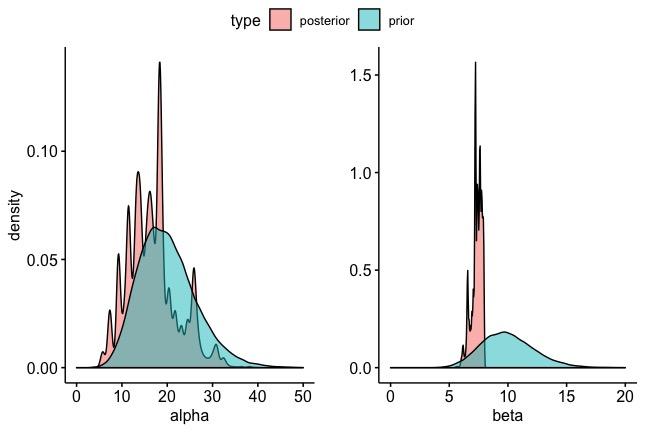
\includegraphics[scale=.30]{prior_post.jpeg}
\caption{Prior and posterior distribution of : $\alpha$ and $\beta$ parameters}
\label{fig:priorpost}
\end{figure}


% how many samples you draw; talk about the posterior distributions; give tables; posterior estimates and quantiles
We obtain 50,000 sample draws from the joint posterior distribution of $\lambda, \alpha$, and $\beta$. As we see in Figure ~\ref{fig:priorpost}, the posterior distribution of $\alpha$ is updated but still on the same range as its prior. However, the posterior distribution of $\beta$ is more concentrated around the left quarter tail of its prior distribution. Note that the model was given two hyperprior distributions for $\alpha$ and $\beta$ s.t. they account for the assumption that on average 20\% of the population in each county contracts coronavirus. We see that this assumption and the Poisson likelihood added their contribution in generating joint posterior and updating prior. 

% table with estimates
\begin{table}
\caption{Posterior mean and variance estimated by Model 1.}
\label{tab:fmodelest}
\begin{center}
\begin{tabular}{ccccc}
\hline
\hline
\\[-5pt]
\multicolumn{1}{c}{Parameter} &
\multicolumn{1}{c}{2.5\%} &
\multicolumn{1}{c}{50\%} &
\multicolumn{1}{c}{97.5\%}\\
\hline
$\alpha$&     7.296&	16.252&  29.445\\
$\beta$&     6.272&    7.410&  7.950\\
\hline
\end{tabular}
\end{center}
\end{table}

% point estimates and the shrinkage
Point and interval estimates of $\alpha$ and $\beta$ are given in Table ~\ref{tab:fmodelest}. The same shrinkage of posterior distribution of $\beta$ can be seen from 95\% credible interval.

% box plots of all lambdas
\begin{figure}[t]
\centering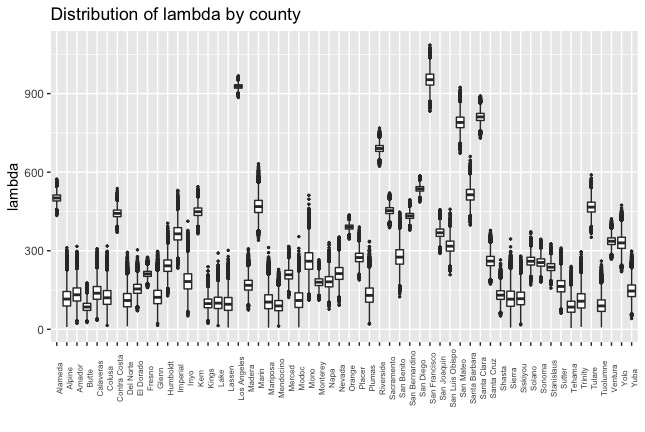
\includegraphics[scale=.31]{lambdas.jpeg}
\caption{Posterior distribution of $\lambda_i$'s depicted by box plots.}
\label{fig:lambdas}
\end{figure}

% for posterior estimates use Gamma's expectation formula !!!
Now we analyze a sample from posterior distributions of each $\lambda_i$ for 58 counties. Figure ~\ref{fig:lambdas} shows the posterior distributions of each $\lambda_i$ for $i = 1, ..., 58$ depicted by box plots. Distribution for Los Angeles is one of the highest and it's also shrunk, comparative to the distribution for San Francisco county, which is of the same height but has more uncertainty. The sampling distribution of $n_i$ is $Poi(\lambda_i c_i / 10^3)$, so that $\lambda_i$ serves as coefficient parameter for each a scaled covariate $c_i/10^3$. For instance, Los Angeles county has population $c_i = 10,039,108$ and hence estimated $E[n_i|\lambda_i]$ is 9,546,425. It means assumption, that 20\% of the population will be infected, combined with observed data estimates infection of 95\% of the Los Angeles population. We also estimate the same rate $\sim 92\%$ for San Francisco county. These estimates are suspiciously high, it might be a lack of fit of data to a model, or we'll to see such high numbers of infection in those counties in the future.

% Are there any substantive differences between counties?
Overall, there is a noticeable difference in posterior distributions of $\lambda_i$'s across counties. Top five counties with the highest quartile 1 in the distribution of $\lambda_i$'s are Los Angeles, San Francisco, San Mateo, Santa Clara, and Riverside. Note that Orange and San Diego counties were among the top five counties with the highest number of infected people per county according to observed data. 


% plot with checks
\begin{figure}[t]
\centering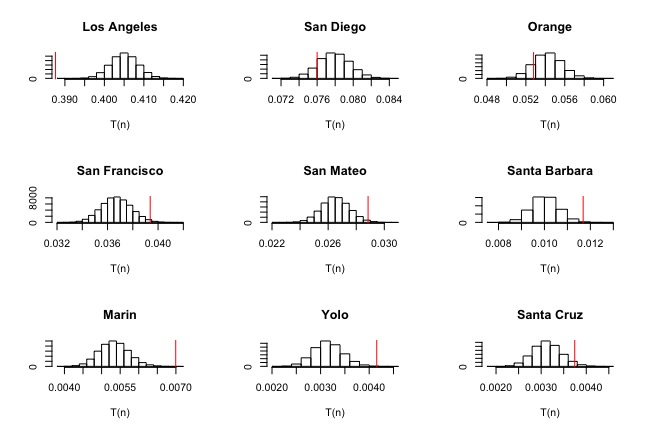
\includegraphics[scale=.30]{quantities.jpeg}
\caption{Distribution of test quantity on replicated data for different counties.}
\label{fig:quantities}
\end{figure}


% Model checks - draw samples from posterior predictive distribution
We draw 1,000 samples from the posterior predictive distribution of $n_i$ for each county. We included the samples of $\theta_i$'s from the previous study's hierarchical model to obtain samples of predictive distribution of the number of deaths. If the model fits the data well, it should be able to replicate data. We noticed in EDA that Los Angeles county has the largest proportion of infections across counties in California. We use this quantity as $T(\mathbf{n}, \lambda)$ and calculate the probabilities of observing more extreme values of it from replicated data for different counties. Counties in Figure \ref{fig:quantities} mostly have some discrepancies from the general trend which is confirmed by posterior probabilities in Table \ref{tab:postprobs}. 

 
 




\subsubsection{Predictive distribution of the number of deaths per 1000 habitants for different counties}

% include plots: Boxplot of deaths
\begin{figure}[t]
\centering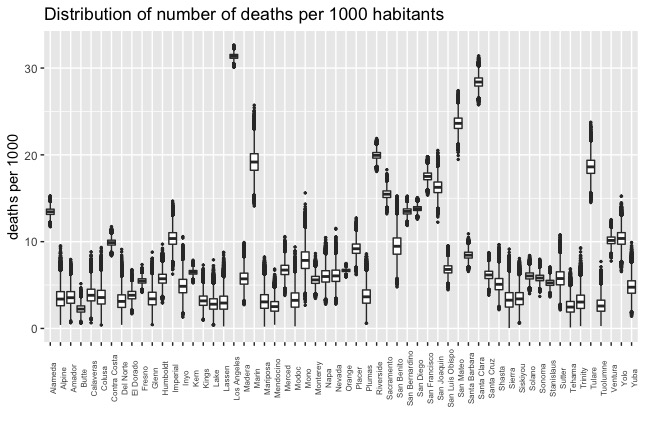
\includegraphics[scale=.30]{deaths1.jpeg}
\caption{Posterior predictive distribution of the number of deaths per 1000 habitants for 58 counties. }
\label{fig:deaths1}
\end{figure}

% intro 
We obtain 50,000 samples of $\tilde{n}_i$ from $p(\tilde{n}_i | n)$ for each county. We also retrieved sample results from previous study: 250 samples of $\theta_i$ from $p(\theta, \mu, \tau | y)$. We combine those sampled to obtain 50,000 samples of the number of deaths per 1000 habitants for each county. Figure ~\ref{fig:deaths1} shows that the distribution of the number of deaths across counties is not homogenous. There are 4 counties with the median number of deaths per 1000 habitants $\geq 20$ and Los Angeles county with the median $\geq 30$. I.e, more than 30 people per 1000 die in Los Angeles due to a novel virus.

Table ~\ref{tab:deaths} shows that more than the number of deaths changed tremendously, as it was impacted by the assumption we gave in prior distribution.








\subsection{Hierarchical Poisson model with Gamma priors (Modified)}
We obtain 50,000 samples from the joint posterior distribution of $\theta, \lambda, \mu$ and $\tau$. Although we are interested in samples of $\theta$ and $\lambda$, we used $\mu, \tau$ as latent variables for an easier sampling procedure from the joint posterior distribution. 

% lambda's plot
\begin{figure}[t]
\centering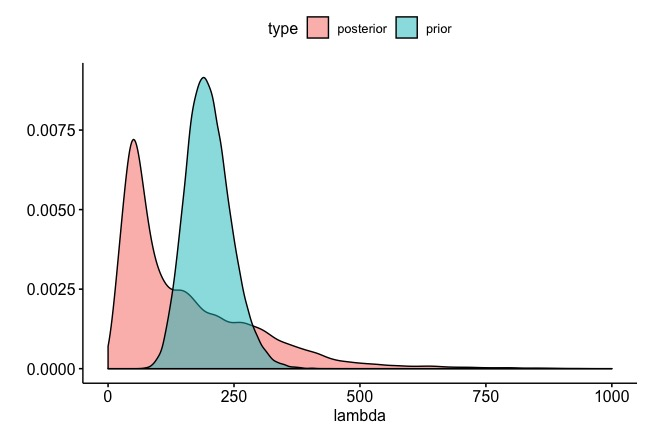
\includegraphics[scale=.30]{lambdass.jpeg}
\caption{Posterior distribution of $\lambda$}
\label{fig:lambdass}
\end{figure}

% report lambdas
Figure ~\ref{fig:lambdass} shows the prior and posterior distributions of $\lambda$ in model 2. The posterior distribution is highly skewed to the right, while prior is more concentrated. The posterior mean of $\lambda$ can be easily calculated since we know its full conditional distribution in a closed form. Hence, $E[\lambda |\mathbf{y, n}] = 154.75$ and 95\% credible interval is $[19.46, 492.97]$. Note that credible is quite wide, which is probably because of a heavy right tail. 

% plot with mortality rates
\begin{figure}[t]
\centering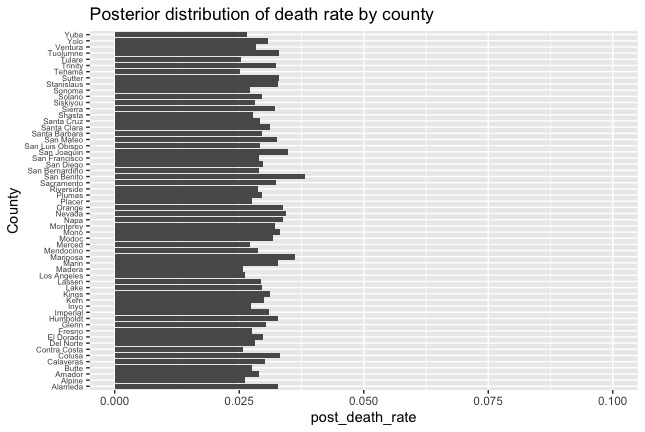
\includegraphics[scale=.30]{postdeaths.jpeg}
\caption{Posterior distribution of mortality rate}
\label{fig:postdeaths}
\end{figure}

% compare mortality rates for each county as in previous study
According to the Figure \ref{fig:postdeaths} the distribution of mortality rate has been homogenized comparative to its distribution in Figure \ref{fig:deathrate}. We set non-informative $Beta(0,0)$ prior for $\mu$, where $\theta_i \sim Be(\theta_i | \mu, \tau)$. So posterior of $\theta_i$ is dominated by the Beta likelihood with combination with data likelihood, which also involve parameter $\theta_i$.

% talk about overall infections and death number -- DELETE if needed
%Remember, we mentioned that $~ 0.6\%$ of people California contracted the virus up to date, and in total, 725 people have died. The overall posterior mean of death rate = $0.0302$, which is multiplied by the total number of people infected in state equals to 733, which is close enough to the true value.

% distribution of number of deaths per 1000 habitants
\begin{figure}[t]
\centering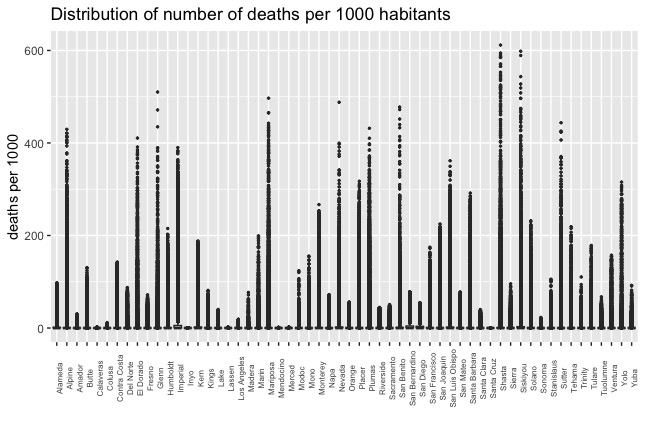
\includegraphics[scale=.30]{deaths2.jpeg}
\caption{Posterior predictive distribution of number of deaths per 1000 habitants.}
\label{fig:postdeathss}
\end{figure}

% compare predictive distribution of the number of deaths per 1000 habitant
We obtain 50,000 samples of $\tilde{n}_i$ and $\tilde{y}_i$ for each county. Using those estimates, we obtain the posterior predictive distribution of the number of deaths. Figure \ref{fig:postdeathss} shows that the distribution of the number of deaths per 1000 habitants is far from being homogenous. We see that almost all distributions are highly skewed with the right heavy tails. We refer to Table \ref{tab:deaths} and see that surprisingly Los Angeles has fewer deaths per 1000 than other counties..

% infection per 1000
\begin{figure}[t]
\centering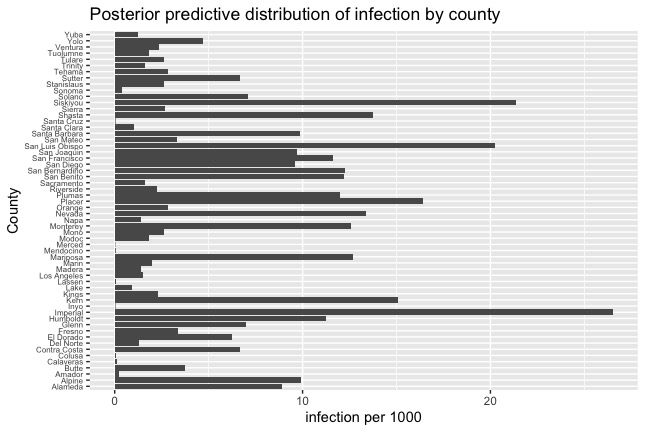
\includegraphics[scale=.30]{infection2.jpeg}
\caption{Posterior predictive distribution of number of infections per 1000 habitants.}
\label{fig:infections}
\end{figure}

% compare predictive distribution of the number of cases per 1000 habitant
We have seen in EDA that the distribution of the number of infections is heterogenous, i.e each county has significantly different (small or high) numbers. We would like to know if this trend is seen in predictions made by model 2. Figure \ref{fig:infections} shows that the distribution is uniform. However, some counties like Imperial, Solano, San Luis Obispo, which had a smaller number of infections tend to have slightly more than the average.

% table with sensitivity results
\begin{table}
\caption{Posterior probability of observing extreme T(n) for Orange county. Calculated by model 2}
\label{tab:orange}
\begin{center}
\begin{tabular}{ccccc}
\hline
\hline
\\[-5pt]
\multicolumn{1}{c}{a} &
\multicolumn{1}{c}{b} &
\multicolumn{1}{c}{T(n)}\\
\hline
20&	10&   0.1342\\
20&     5&  0.1265\\
5&	5& 0.4226\\
0.5&     0.5&  0.4927 \\
\hline
\end{tabular}
\end{center}
\end{table}


% Sensitivity analysis -- MODIFY
As you see from the table our quantity of interest is affected by a change in the values of $a$ and $b$. As their values decrease we see better fit (in terms fo Orange county only). So we have to be very careful in the choice of hyperparameter values. We can evaluate sensitivity w.r.t. other test quantities or aspects of the data.








\subsection{Comparing two models}
We fit five models in total to the COVID-19 data. The last three models are hierarchical, and the last two treat the total number of infected people $n_i$ in each county as a random variable rather than fixed. The last model also takes into account potential overdispersion in the number of deaths. 

% report posterior distribution of deaths per 1000 habitants
\begin{table}
\caption{Distributions of the number of deaths per 1000 habitants for each county. Estimated by model 1 \& 2}
\label{tab:deaths}
\begin{center}
\begin{tabular}{ccccc}
\hline
\hline
\\[-5pt]
\multicolumn{1}{c}{County} &
\multicolumn{1}{c}{$E_{1}[\tilde{y}|y]$} &
\multicolumn{1}{c}{$E_{2}[\tilde{y}|y]$} &
\multicolumn{1}{c}{y}\\
\hline
Los Angeles&	31.35&   0.610 & 0.032\\
Santa Clara&     28.39&  0.402 &	 0.031\\
San Mateo&	23.64& 1.309	& 0.027\\
Riverside&     19.95&  1.270 & 0.021\\
Marin&     19.20& 0.824 & 0.038\\
\hline
\end{tabular}
\end{center}
\end{table}

% comment on the table above
We see in Table \ref{tab:deaths} the predictive distribution by model 1 was influenced by the assumption that the mean number of cases is equal to 20\% of the population. Model 2 has also overestimated the mean number of deaths comparative to a summary from observed data. On average, it's expected that the number of deaths per 100 habitants is between 5 and 14 (for counties in the table) by model 2, while the number of deaths per 1000 habitants is between 20 and 31 by model 1.


% table with probs from PPC
\begin{table}
\caption{Posterior probability of observing extreme T(n) calculated by model 1 \& 2}
\label{tab:postprobs}
\begin{center}
\begin{tabular}{ccccc}
\hline
\hline
\\[-5pt]
\multicolumn{1}{c}{County} &
\multicolumn{1}{c}{Model1} &
\multicolumn{1}{c}{Model 2}\\
\hline
 Los Angeles&	0.0000 &	0.0883\\
San Diego & 0.1368 &	0.3887\\
Orange & 0.1648 & 0.1342 \\
San Francisco & 0.0130  & 0.2225\\
San Mateo & 0.0107 & 0.1146\\
Santa Barbara & 0.0028 & 0.2313\\
Marin & 0.0001 & 0.0517\\
Yolo & 0.0009 & 0.1373\\
Santa Cruz & 0.0299 & 0.0009\\
\hline
\end{tabular}
\end{center}
\end{table}


% report predictive distribution checks
We draw samples from posterior predictive distribution of the number of infected people in each county to see if models were able to replicate the observed data. Initially, we observed that Los Angeles county had the highest number of infected people across all 58 counties, and we want to know if the same trend is the case for both models. Posterior probabilities of observing as extreme values as a test quantity are given in Table \ref{tab:postprobs} for both models. Note that we also test other counties, which have unusual behavior in the distribution of the number of infected people. Posterior probabilities calculated by model 2 are slightly better than in model 1. However, there is no major improvement except for counties like San Diego, San Francisco, and Santa Barbara.


% report comparisons table: DIC, Gelfand-Ghost
\begin{table}
\label{table:anan}
\caption{Model fit assessment}
\begin{center}
\begin{tabular}{ccccc}
\hline
\hline
\\[-5pt]
\multicolumn{1}{c}{Model} &
\multicolumn{1}{c}{DIC} &
\multicolumn{1}{c}{Gelfand-Ghost}\\
\hline
 Model 1&	294.13&	1.005e+14\\
Model 2&	-9182.21&	1.321e+10\\
\hline
\end{tabular}
\end{center}
\end{table}

% discuss table above
We employ two different methods to compare the models, and probably find a better fit. We also used two criteria to choose between models. Gelfand \& Ghosh criteria compare the predictive abilities of two models. Although the criteria values are very high for both models, the second modified model has substantively smaller criteria value. Also, we employed DIC, which is a generalization of AIC for hierarchical models. It's calculated by estimating the effective number of parameters in the model. We know that negative DIC values are legit and small values of DIC are preferred. Hence, by both criteria model 2 seems to be a better fit for the COVID-19 data than model 1. 


% overall computational performance
There was a tremendous difference in the computation time of two models for obtaining samples from posterior. I.e model 2 required 3 times more time than model 1 for the same number of samples. Since we employed a combination of Metropolis-Hastings algorithm and rejection algorithms for model 2, it required more time to run 5 chains and obtain 50,000 samples from posterior. That time requirement triples since we obtain samples of $\tilde{n}_i$ and then samples of $\tilde{y}_i$ for each county. 

% model complexity 
Although the second model is more complex, it was easier to obtain full conditionals and construct a working sampling algorithm. We could use Gibbs sampler for the first model as well if we treated $\lambda_i$'s as a latent variable. Our approach was to use the Griddy approach to sample from $p(\alpha, \beta | mathbf{n})$ which created a lot of computational issues so we manually simplified the kernel of $p(\alpha, \beta | mathbf{n})$ and wrote many additional functions to evaluate density only. 


















\section{Discussion} 

% intro
We employed two different constructions of the Poisson-Binomial models. We treated the number of infected people as a random variable along with the number of deaths per county. Our preliminary results showed that the infection rate and death rate across counties are not homogenous. It was also confirmed throughout by fitting the two models above. 

% Talk about future: time when will we reach that 20%, how to slow the spread and find the patterns in different counties
We assumed that $20\%$ of people in California will contract the virus. Actually we used it as a piece of prior information in the first model and used it indirectly in the second model as well. We ignored the time feature of the spread of the virus, i.e we are not interested in estimating when will those $20\%$ be infected. So it can be the next step to include time in our model. 

% Time-space varying parameter
As a next step, we can consider a model that accounts for the time and space varying nature of the spread of the virus. I.e we might want to employ Gaussian or Poisson processes that are suitable for time series as well as spatial data. 




%Note:BibTeX also works

\begin{references}
\itemsep=0pt
{\footnotesize

\item
Aljazeera, News
\\\url{https://www.aljazeera.com/news/}

\item
Hines B 2019, Population Density of California
\\\url{https://storymaps.arcgis.com/stories/252b65cbe331420389c61453c61ea221}

\item
Kuttubekova G 2020, Bayesian Analysis of COVID-19 cases in California
\\\url{https://github.com/kgulzina/bayesian-analysis-of-COVID19-in-CA}

\item 
Worldometer: Coronavirus,
\\\url{https://www.worldometers.info/coronavirus/}


% add BDA book
\item 
Gelman, A., Carlin, J. B., Stern, H. S., Dunson, D. B., Vehtari, A., \& Rubin, D. B. (2013), $\textit{Bayesian Data Analysis} (3^{rd}$ ed.). CRC Press. Taylor \& Francis Group.


}
\end{references}


\end{document}


